\documentclass[11pt, a4paper, oneside, parskip=full-]{scrartcl}

% -- PREABLE

% global settings
\renewcommand\labelitemi{-}

% packages
\usepackage[utf8]{inputenc}
\usepackage{graphicx} % to embed figures
\usepackage{float} % use [H] to place fig exactly where specified in code
\usepackage{tabularx} % table with columns that fill width of page using X
\usepackage{booktabs} % table utilities like \midrule
\usepackage{multirow} % span multiple rows in table
\usepackage{enumitem} % pass key-value config to itemize and enumberable
\usepackage{hyperref} % for links and urls
\usepackage[style=numeric,backend=biber,sorting=none]{biblatex} % For citing
\usepackage{listings} % For code snippets
\usepackage{rotating} % To turn images 90 degrees

\addbibresource{thesis.bib}

\graphicspath{ {img/} } % path where grahics are stored

% title page parameters
\title{Open-Source GIS Sandbox \& Data Stories - New tools for workshop interactivity}
\author{Marc Folini}
\date{May 2022}

% -- BODY
\begin{document}

%-------------
% TITLE, ABSTRACT
%-------------
\begin{titlepage}
\pagenumbering{Roman}
\setcounter{page}{1}
% create title page
\clearpage\maketitle
\thispagestyle{empty}
% abstract
\begin{abstract}
GIS workshops benefit from supplementing theoretical concepts with exercises for
participants to become an active part in the learning experience. This requires
participants to have access to an environment that provides the necessary
software and data - ideally with minimal setup effort, independent of the system
they use and easy to uninstall without leaving traces after the workshop.
Different approaches were evaluated, and container technology was found to be a
good fit to abstract away the hassle of setting up the tools and infrastructure.
A proof of concept of what will be referred to as \emph{Sandbox} was implemented
and made publicly available free to use under MIT license. The Sandbox is based
on Docker Compose and provides access to a spatial database, an OGC data server,
GDAL and Python scripting capabilities with access to libraries from the
geo-ecosystem. It requires only minimal setup and only a single command to be
started and stopped respectively.\\

In order to help participants to make sense of the Sandbox components and their
interactions the concept of \emph{data stories} was explored. Designed as
data-driven cross-application tutorials, they allow participants to fully focus
on how different applications interact to transform raw data into meaningful
results. This is in contrast to many other tutorials, to which data is secondary
to teach tool-centered functionalities in a narrow scope. Built upon the Sandbox
capabilities, an example data story was implemented to create a bike suitability
map from raw open data from the city of Zürich. Participants learn about the
GDAL command line tools to inspect datasets and load them into PostGIS, where
spatial processing and aggregation is performed. The result is made available as
a new dataset to be consumed and styled in QGIS.
\end{abstract}
\end{titlepage}

%-------------
% TABLE OF CONTENT
%-------------
\newpage
\tableofcontents

%-------------
% INTRODUCTION
%-------------
\newpage
\pagenumbering{arabic}
\setcounter{page}{1}
\section{Introduction}

The GIS\footnote{Geographic Information System (GIS).} ecosystem today is
extensive and fast evolving with multiple technologies addressing similar use
cases with varying overlap in functionality. The motivation to employ GIS
technology is often data-driven, i.e. a company usually wants to gain insights
from spatial data or process it to be used downstream in products. This requires
an end-to-end understanding how different components of the GIS ecosystem
interact to transform the raw data into the desired product. For somebody new to
the field, the vast amount of possibilities might be overwhelming at best and
frustrating at worst when trying to develop a holistic mental model about what
technologies to use in what way to tackle real world use cases.

Many tutorials exist, but these are usually centered around a specific tool or
technology, whereby data is of secondary nature to explain the functionalities
in a narrow scope. Workshops and lectures are another common vehicle to acquire
knowledge about a field, whereby is desirable for participants to experience
theoretical concepts hands-on for themselves. The challenge lies in providing
all participants with access to the respective software and data with minimal
setup efforts. There is a shortcoming of such solutions, particularly when it
comes to more complex setups with multiple components that need to interact.

This thesis was written as part of the CAS RIS 2021/22\footnote{Certificate of
advanced studies (CAS) in GIS (in German RIS) offered by ETH Zurich.}. It was
hypothesized that there is a gap between what people new to the field and
organizers of lectures and workshops need and what is widely available. This
thesis addressed this gap on two levels:
\begin{enumerate}
  \item \textbf{Infrastructure} In order to provide participants access to a
  variety of components from the GIS ecosystem with minimal setup effort the
  concept of a \emph{Sandbox} environment was explored. The requirements and
  components to be implemented were chosen to support the CAS RIS course
  curriculum.
  \item \textbf{Content} In order to help participants to make sense of the
  Sandbox components and their interactions, the concept of a \emph{data story}
  was explored. Each data story is a data-driven cross-application tutorial. It
  has a tangible data driven use case and provides guidance on how available
  technologies and tools interact with the data to achieve the desired result.
  An example data story was conceptualized and implemented to create a bike
  suitability map from raw open data from the city of Zürich. Participants learn
  about the GDAL command line tools to inspect datasets and load them into
  PostGIS, where spatial processing and aggregation is performed. The result is
  made available as a new dataset to be consumed and styled in QGIS.
\end{enumerate}


%-------------
% SANDBOX
%-------------
\section{Sandbox}

% Requirements
%-------------
\subsection{Requirement analysis} \label{sectionrequirements}

The content of the CAS RIS course was analyzed for potential hands-on exercises.
From these findings functional and non-functional
requirements\footnote{Functional requirements specify the tasks an application
must be able to perform. Non-functional requirements specify additional aspects
about the application performing the task, for example usability, look and feel
or performance. } for a Sandbox were then derived.

% Content analyis
%-------------
\subsubsection{Curriculum analysis}
At the time of writing the CAS curriculum consisted of four weeks of content
modules on a wide variety of topics. Each module was screened with a focus on
where a Sandbox could facilitate hands-on experiences without substantially
altering the module structure or material. Modules focusing primarily on usage
of proprietary software like ArcGIS were ignored. Table
\ref{tab:tContentAnalysis} shows the results of the analysis.

\begin{table}[!htbp]
  \centering
  \caption{Content analysis of existing lectures for Sandbox facilitation potential.}
  \label{tab:tContentAnalysis}
  \begin{tabularx}{\textwidth}{lX}
    \toprule
    % header row start
    \textbf{Module} & \textbf{Sandbox facilitation potential} \\
    \midrule
    % row start
    Interoperabilität &
      \begin{itemize}[left=0pt,nosep,before={\begin{minipage}[t]{\hsize}},after
      ={\end{minipage}}]
      \item Inspection of and conversion between various data formats.
      \item Read Shapefile into a spatial database.
      \end{itemize}\nointerlineskip\\
    \midrule
    % row start
    SQL & Write and run basic SQL queries on sample data. \\
    \midrule
    % row start
    Geodatenbanken &
    \begin{itemize}[left=0pt,nosep,before={\begin{minipage}[t]{\hsize}},after
    ={\end{minipage}}]
      \item Run basic spatial queries on sample data.
      \item Perform spatial aggregation on sample data.
      \end{itemize}\nointerlineskip\\
    \midrule
    % multirow(4) start
    Geometrische Methoden & \multirow[t]{4}{*}{Run simple examples on sample
    data.} \\
    \cmidrule(r){1-1} Topologische Methoden &  \\
    \cmidrule(r){1-1} Mengenmethoden &  \\
    \cmidrule(r){1-1} Statistische Methoden &  \\
    \midrule
    % row start
    Einführung in Python & Self-study introduction of Python basics. \\
    \midrule
    % row start
    Internet und GIS I \& II &
      \begin{itemize}[left=0pt,nosep,before={\begin{minipage}[t]{\hsize}},after
      ={\end{minipage}}]
      \item Load data from OGC web services WMS/WFS/WCS.
      \item Consume WMS with an OGC compliant client system.
      \end{itemize}\nointerlineskip \\
    \midrule
    % row start
    Projekt Internet \& GIS &
      \begin{itemize}[left=0pt,nosep,before={\begin{minipage}[t]{\hsize}},after
      ={\end{minipage}}]
      \item Use geodatabase as data source for OGC server.
      \item Create style and serve data as WMS.
      \item Consume WMS with an OGC compliant client system.
      \end{itemize}\nointerlineskip \\
    \bottomrule
  \end{tabularx}%
\end{table}%

% Functional requirements
%-------------
\subsubsection{Functional requirements}
The following functional requirements were identified for the Sandbox to be
useful in realizing the potential identified in the curriculum analysis:
\begin{itemize}
  \item A spatial database is available together with utilities to import and
  query data.
  \item An OGC\footnote{The Open Geospatial Consortium (OGC) is a worldwide
  community to improve the access to geospatial data by various means such as
  developing standards. Such standards for the web include Web Map Service
  (WMS), Web Feature Service (WFS) and Web Coverage Service (WCS) to load styled
  map images, simple geometry features and raster data via HTTP respectively.}
  server implementation is available. There is a way to read predefined example
  data, read data from the user's system or connect to the Sandbox spatial
  database.
  \item An OGC client implementation is available, which can interact with the
  Sandbox OGC server or any other OGC service publicly available on the
  internet.
  \item GDAL\cite{gdal} command line utilities such as gdalinfo, ogrinfo and
  ogr2ogr are available. There is a way to read either predefined example data
  or read data from the user's system.
  \item An environment is available to write and run Python scripts which make
  use of the Python geo-ecosystem. A use case would be to provide illustrative
  examples for the concepts of geometry, topology and spatial statistics.
\end{itemize}

% Non-Functional requirements
%-------------
\subsubsection{Non-Functional requirements}
\begin{itemize}
  \item Users can create content which is persisted between usages of the
  Sandbox.
  \item There is a possibility to ship example scripts and data as part of the
  Sandbox.
  \item Creation and distribution of data stories that are compatible with the
  tools of the Sandbox should be possible without in-depth technological
  knowledge.
  \item The Sandbox can be installed effortlessly and in a uniform way across
  the most common operating systems, namely Apple OS, Linux and Windows.
  \item The Sandbox can be uninstalled without leaving traces on the operating
  system.
  \item Turning the Sandbox on/off and accessing components should not require
  any programming knowledge.
  \item A partial or total reset of applications and data is possible in case
  something gets messed up.
  \item Usage is not coupled to the duration of the CAS RIS course or otherwise
  restricted (e.g. via externally controlled credentials).
\end{itemize}

% Existing projects
%-------------
\subsection{Existing projects}
Google search engine was used to look for already existing similar projects
using various combinations of the terms \emph{gis}, \emph{geo}, \emph{sandbox},
\emph{workshop}, \emph{playground} and \emph{spatial}. No project was found that
satisfied the requirements outlined in section \ref{sectionrequirements}, but
some noteworthy findings are listed below.

\begin{itemize}
  \item Joeyklee's Geosandbox\cite{project-joeyklee} consists of tutorials that
  focus on JavaScript client side mapping libraries such as Leaflet. It is not
  suitable for our purpose but mentioned here to avoid confusion due to the very
  similar name.
  \item IDRE Sandbox\cite{project-idre} does not provide any easy access to
  tools, but seems to be a collection of workshops and tutorials. It is
  mentioned here because the interesting goals and presentation of some
  workshops served as inspiration for the data story of this thesis.
  \item Digital Earth Australia (DEA) Sandbox\cite{project-dea} was a wonderful
  discovery. After creating a free account a cloud hosted
  JupyterLab\cite{jupyterlab} platform with extensive Python Jupyter Notebooks
  provide an interactive engaging experience to learn about the analysis of
  satellite imagery and much more. The DEA Sandbox was a major inspiration for
  the heavy focus use of JupyterLab in our Sandbox.
  \item Geopython Workshop Repository\cite{project-geopython} is an extensive
  knowledge hub about a broad range of geospatial topics. The workshop is built
  on Python Jupyter Notebooks using a containerized JupyterLab environment with
  pre-installed libraries. Docker Compose\cite{dockercompose} is used as
  container orchestration technology. Even though the setup is too limited for
  the use case of this thesis (a spatial database is missing for example) the
  idea of using container technology to abstract away dependency management
  provided major inspiration for this thesis.
\end{itemize}

% Technology evaluation
%-------------
\subsection{Technology evaluation}

\subsubsection{Container terminology by the example of Docker}
Container technology has been around for decades but took off in 2013 with the
release of Docker, which provided the tools that made container technology
accessible to the broader mass. The basic idea is to package applications, so
they can be run in isolation from other applications. Compared to virtual
machines containers are very lightweight and can be started and stopped within
seconds.

In Docker terminology, the first step towards packaging an application is to
create a \emph{Dockerfile}, a text file which describes the installation
procedure and configuration in a standardized way. A Dockerfile is used to
\emph{build an image}, a lightweight, standalone, executable package of software
that includes everything needed to run an application: code, runtime, system
tools, system libraries and settings\cite{dockerimage}. From an image one or
more \emph{containers} can be created which provide an isolated environment
within which the containerized application runs.

\subsubsection{High level architectural approaches}
The research on existing projects and further exploration of potential
technologies led to three distinct groups of architectural approaches to be
evaluated: Sandbox as direct installation on user system, Sandbox as local
containerized application and Sandbox as cloud service.

\subsubsection*{Sandbox as direct installation on user system}
It was found that only four established open-source projects (QGIS\cite{qgis},
PostGIS\cite{postgis}, pgAdmin\cite{pgadmin} and GeoServer\cite{geoserver})
would be enough to satisfy the major part of the functional requirements. While
the roles of PostGIS as spatial database and GeoServer as OGC data server are
well-defined, the QGIS installation is particularly interesting because it comes
bundled with versions of GDAL and Python that work together well. The community
has produced installers for all major operating systems, which makes the
installation relatively straight-forward.

When it comes to non-functional requirements this approach falls short. A major
shortcoming is the lengthy and intrusive setup stemming from the lack of
separation of the Sandbox software from the rest of the user's system. Depending
on already existing software and specific configurations this approach is at
best error-prone and at worst capable to permanently alter the user's system.
Because with this approach only the tools themselves are installed, tutorials
and data stories would need to be provided in a separate way. On a positive
note, the installed tools could be used beyond the duration of the CAS RIS
course without problems and the decoupling of the distribution of tutorials and
data stories makes it easy to be updated without technical knowledge.

\subsubsection*{Sandbox as local containerized application}
Container technology has been around for decades but took off in 2013 with the
release of Docker, which provided the tools that made container technology
accessible to the broader mass. The basic idea is to package applications, so
they can be run in isolation from other applications. Compared to virtual
machines containers are very lightweight and can be started and stopped within
seconds.

This approach takes the direct installation approach one step further by running
a spatial database and an OGC data server as containerized applications isolated
from the host system. A difference from the direct installation approach is that
QGIS was found to be not suitable for this approach because of extra
configuration required for graphical output on the host system (the computer the
containerized applications run on). On a positive note, complex installation
procedures for containerized applications can be fully abstracted away from the
user during the packaging process. This would allow for example to fulfill the
functional requirements without QGIS by setting up JupyterLab environment with
system dependencies like GDAL in order to have access to a wide variety of
Python packages from Python's geo-ecosystem and GDAL terminal commands.
Containers can also contain data which optionally can be persisted on the host
on virtual volumes. Example scripts and data stories can be distributed as part
of the container and by using volumes they can be persisted across Sandbox
restarts or selectively reset.

An initial setup complexity is the installation of a container runtime, here
Docker\footnote{Any other software that provides a container runtime will do to
run containerized applications. Up to this day Docker remains one of the most
popular tools for that purpose to the point where it is often used synonymously
for everything to do with containers. Docker is chosen for its maturity and
excellent documentation.}, on the user's computer, which is an easy and mature
process for all major operating systems at this point.

\subsubsection*{Sandbox as cloud service}
The advances of container technology went hand in hand with the maturation of
the publicly available cloud. It's possible today even for a layman to run
containerized applications in the cloud at scale using a variety of managed
services ranging from authentication to load balancing.

This approach takes the local containerized approach one step further into the
cloud. Instead of bothering with the installation of Docker on the user's
computer and running the containers locally the Sandbox is made available as a
service with a simple web interface and optionally some kind of login. Some
functional requirements such as the availability of a spatial database could
even be satisfied with cloud native components such as fully managed database
services.

The advantage of a cloud service is the low entry barrier because there is no
installation required. Example data and data stories can be made readily
available as part of the container setup and resetting is as simple as starting
a new Sandbox cloud instance. But this convenience comes with a cost and
complexity overhead at the cloud side, because for persisting data across
sessions some form of authentication must be in place and every cloud session
uses resources which are billed by the second. Assuming the cloud Sandbox is
publicly available to fulfill the requirement that the Sandbox' usage should not
be coupled to the duration of the CAS RIS course, further complexity arises from
implementing and maintaining security best practices against malicious attacks.
Data management is another topic which can prove challenging when it comes to
cloud services in the geospatial domain, because data usually needs to be
uploaded before being accessible and spatial data can quickly become rather
large for standard internet connection upload speeds leading to disruptions and
waiting times.

\subsubsection*{Conclusion: Sandbox as local containerized application}
All three approaches satisfy the functional requirements, so the non-functional
requirements will be used to argue for the final decision. The direct
installation approach falls short here. The local containerization approach has
some minor shortcomings when it comes to the initial installation, but shines in
almost all other areas. The cloud service approach is the opposite, shining with
a zero-effort setup but falling behind the local containerization approach in
terms of maintainability, cost, and data management.

The approach \emph{Sandbox as local containerized application} was eventually
chosen for further implementation, because the simplicity of a local setup
combined with the advantages of container technologies was found to outweigh the
cost of the initial setup.

\subsubsection{Technology evaluation for local containerized application}
The technology has to be able to run multiple containerized applications which
can communicate among each other as well as with the host system and store data
which is persisted across Sandbox restarts. Among many possibilities, three
technologies were considered more closely due to their popularity and the
availability of detailed documentation: Docker Compose, Docker Swarm and
Minikube.

\begin{itemize}
  \item \textbf{Docker Compose} orchestrates multiple containerized applications
  on a single host to act like a single application, whereby a simple text file
  specifies details about the components and their interactions.
  \item \textbf{Docker Swarm}\cite{dockerswarm} shares many concepts with Docker
  Compose and can be considered an evolution towards orchestrating multiple
  containerized applications across multiple host machines. It is also possible
  to run Docker Swarm on a single host machine.
  \item \textbf{Minikube}\cite{minikube} is a tool that lets you run a local
  version of a Kubernetes Cluster. Kubernetes is one of the most popular
  container orchestration software and at a high level similar to Docker Swarm.
  It provides its own approach towards managing containers, networking and
  storage which is generally more geared towards large-scale enterprise
  applications.
\end{itemize}

All three technologies were evaluated on a two container setup of a spatial
database (PostGIS) and an associated administrator application (pgAdmin). While
all three technologies provided extensive documentation that allowed for
successful testing, Docker Compose was found to be the simplest solution in
terms of initial setup and ease of use, due to its single configuration file and
the targeted use case to run on a single host. To that end \emph{Docker Compose}
was chosen as the technology to implement the \emph{Sandbox as local
containerized application}.

% Architecture
%-------------
\subsection{Architecture}
The Sandbox was designed as a modular multi-container setup to be run locally by
Docker Compose. The architecture is outlined in Figure \ref{fig:sandboxsetup}
and will be explained in the following sections. \\

 \begin{sidewaysfigure}
  \centering
  \begin{figure}[H]
    \centering
    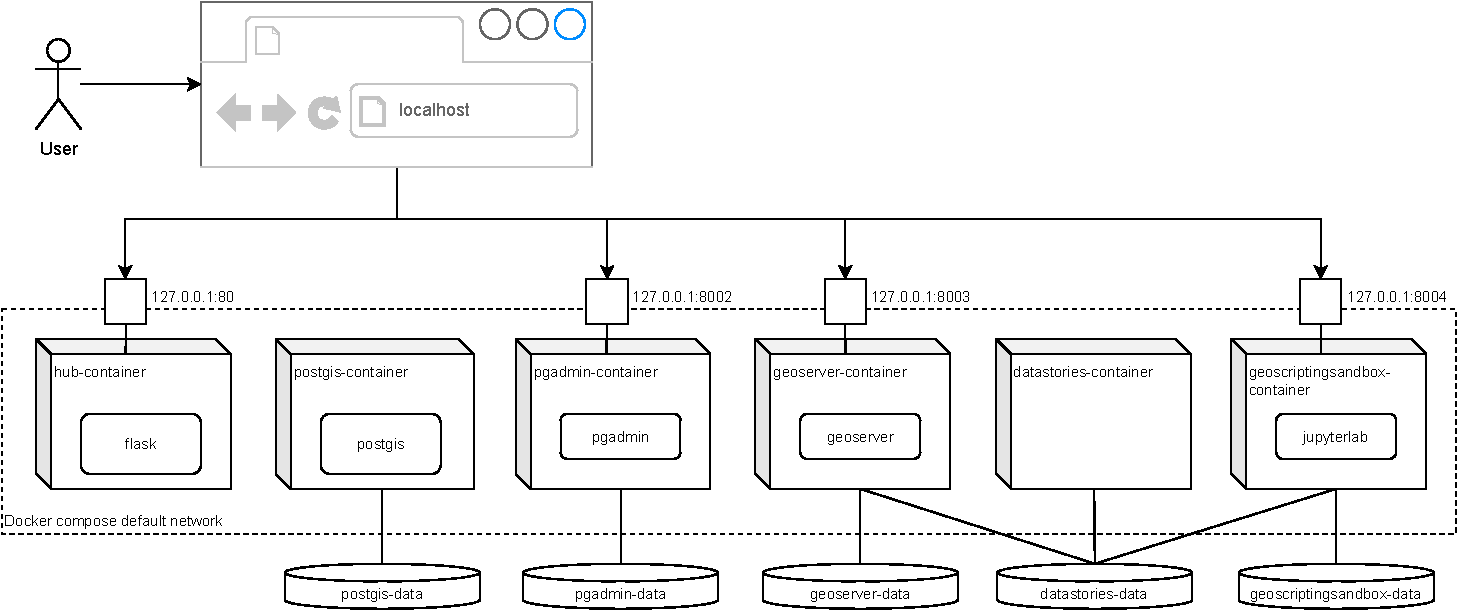
\includegraphics[width=1\textwidth]{composeSetup}
    \caption{Sandbox Docker Compose architecture}
    \label{fig:sandboxsetup}
  \end{figure}
\end{sidewaysfigure}

\subsubsection*{Terminology of Docker and Docker Compose}
In Docker terminology, the first step towards packaging an application is to
create a \emph{Dockerfile}, a text file which describes the installation
procedure and configuration of the desired application package in a standardized
way. A Dockerfile is used to \emph{build an image}, a lightweight, standalone
package of software that includes everything needed to run an application: code,
runtime, system tools, system libraries and settings\cite{dockerimage}. An image
is a template which can be easily distributed and from which one or more
\emph{containers} can be created within which the containerized application runs
in its isolated environment.

Docker Compose orchestrates multiple containerized applications on a single host
to act like a single application. At the heart of a Docker Compose application
is a configuration file, called \emph{compose-file} which describes the
components of the multi-container setup and how they interact. Each component is
called a \emph{service}, which consists of an image that specifies the
containerized application at the heart of the service and additional
configuration about how to interact with other services and the host system.
When a Docker Compose application is started, the images of each service are
used to create containers within which the application of interest then runs. A
compose-file can also declare \emph{volumes}, which can be used by services to
save data which should be persisted across restarts of a service and
\emph{network settings}, which define how containers can interact with each
other and the host network.

\subsubsection*{Containerized applications}
At its heart the Sandbox consists of six services, each defining a container
with a distinct purpose:

\begin{itemize}
  \item \textbf{hub-container} runs a simple Python Flask\cite{flask} web
  application that serves as an entry point and central hub for the Sandbox.
  Here a user finds links to access other Sandbox components and the relevant
  connection information. This \emph{Sandbox Hub} is the first thing a user sees
  when typing \emph{localhost} in the browser after starting the Sandbox.
  \item \textbf{postgis-container} is a containerized version of PostGIS, a
  spatial database.
  \item \textbf{pgadmin-container} is a containerized version of pgAdmin4, a
  graphical user interface to facilitate the administration of PostgreSQL based
  databases, such as PostGIS.
  \item \textbf{geoserver-container} is a containerized version of GeoServer,
  which is an OGC data server and a reference implementation of the OGC web
  services.
  \item \textbf{content-container} serves solely as a data storage without any
  containerized application. It contains the data story related narrative in
  form of Jupyter Notebooks as well as the sample data.
  \item \textbf{jupyterlabgeoenv-container} is a containerized version of
  JupyterLab, a web-based interactive development environment for Python scripts
  and more. It should come bundled with various pre-installed Python packages
  from the geo-ecosystem and fundamental libraries such as GDAL and
  GEOS\cite{geos}. This setup allows users to explore the Python geo-ecosystem
  as well as the various command line utilities that GDAL offers. The expressive
  nature of Jupyter Notebooks is also used to visualize the data stories.
\end{itemize}

\subsubsection*{Usage of volumes for persistent data storage}
Some containers make use of virtual volumes as shown in Figure
\ref{fig:sandboxsetup} to persist data across restarts of the Sandbox. Examples
include the data stored in PostGIS, the database connections set up in pgAdmin
or the data and configuration files used by GeoServer. A special case is
content-data, which can be accessed by other containers such as
jupyterlabgeoenv-container to access the data story Jupyter Notebooks.

\subsubsection*{Networking}
All containers are part of a virtual network managed by Docker Compose which is
isolated from the host system. In this network every container can connect to
every other container by its container name and the port exposed by the
container's application. As shown in Figure \ref{fig:sandboxsetup} some
containers also expose selected ports to the host network, which allows to
establish a connection to the application in the container from outside the
Docker Compose network through the host network's localhost interface.

\subsubsection*{Access to host file system}
Even though not indicated in Figure \ref{fig:sandboxsetup}, it is also possible
to grant containers access to the file system of the host machine. This seems to
contradict the basic idea of isolation but proves to be useful in certain cases.
The current Sandbox implementation creates such a link to the host file system
for the jupyterlabgeoenv-container and geoserver-container with the intent to
make it easy for users to let these components make use of data saved on their
local machine.

% Implementation
%-------------
\subsection{Implementation}

This section covers the implementation of the Sandbox using Docker Compose. The
resulting implementation is provided in this thesis'
repository\cite{osgeostacksandbox} and is free to use under MIT license.

\subsubsection*{Containerized applications}
In a first step, a search was performed on DockerHub\cite{dockerhub}, an online
repository for image distribution. For the following containerized applications
of our architecture suitable third-party images were available and the image
names with appropriate versions were added to the compose-file:

\begin{itemize}
  \item For postgis-container the official PostGIS image was
  used\cite{postgis-container}.
  \item For pgadmin-container the official pgAdmin4 image was
  used\cite{pgadmin-container}.
  \item For geoserver-container a GeoServer image provided by Kartoza was
  used\cite{geoserver-container}. This image has configuration options to
  include community extensions, plugins and sample data.
\end{itemize}

For each of the other required containerized applications a suitable Dockerfile
was created describing how to build an image containing the desired application
and data. GitHub Actions\cite{githubactions} were used to create automated
workflows to build images from the Dockerfiles and upload them to GitHub
Container Registry\cite{gcr}, GitHub's image distribution platform. The image
name with appropriate version was then added to the compose-file.

\subsubsection*{Configurable compose-file}
It was deemed important to let users easily configure parts of the Sandbox. For
example, the default ports exposed by the Sandbox for external connections might
clash with those of other pre-installed software on the host. The Sandbox
implements a standard Docker Compose pattern, whereby variables with default
values are used in the compose-file, which can be selectively overwritten by
creating an environment file\cite{composeenvfile}. A complete list of variables
can be found in the Sandbox repository top level README\cite{osgeostacksandbox}.
In order to reflect changes that impact how to connect to a container in the
Sandbox Hub, its content is almost entirely specified in the compose-file using
the same variables.

\subsubsection*{Configurable Python environment in JupyterLab-GeoEnv}
The Python environment in JupyterLab-GeoEnv comes with a broad range of packages
pre-installed in the image, which results in a fast startup but does not allow
persisting user changes such as package additions or modifications. Persisting
the whole Python environment on a volume would allow the user to persist all
modifications, but with the downside that reproducibility is not necessarily
given which can lead to problems when moving to a new version of
JupyterLab-GeoEnv. A compromise solution was implemented, whereby the user can
specify additional packages in a dedicated standardized requirements
file\cite{piprequirementsfile}. At each Sandbox startup the user defined
packages are lost (because the Python environment is not persisted on a volume),
but the content of the file is re-installed on top of the base environment. The
package archives are downloaded and persisted on a volume on first installation,
which allows subsequent installations from these archives even without internet
connection. One downside with this approach is that each user package increases
the startup time of JupyterLab-GeoEnv, because it is only available to users
after the package installation completed. This sequential nature was a
deliberate design decision, because the alternative where the installation
happens in the background could easily lead to strange behavior when the user
tries to run code that requires a user specified package that has not yet been
installed in the background.

\subsubsection*{Networking and user experience challenge}
Containers interacting with each other use the Docker Compose network, while all
connections from outside the Sandbox are routed via the host's localhost
interface. For the user this means that the way to connect to a Sandbox
container differs based on whether the connection happens from another Sandbox
container (e.g. Sandbox pgAdmin to Sandbox PostGIS) or from outside the Sandbox
(e.g. QGIS to Sandbox PostGIS). Hours were spent researching how to homogenize
the user experience without success and in the current implementation the
Sandbox Hub makes it as explicit as possible which connection information to use
in which case.


% Using the Sandbox
%-------------
\subsection{Setup and usage}
For a more detailed documentation on how to set up and use the Sandbox please
refer to the top level README page of this thesis'
repository\cite{osgeostacksandbox}.

\subsubsection*{Initial setup}
The only prerequisite to use the Sandbox is a working installation of Docker,
which has become a straight-forward task across all common operating systems in
recent years by the maturation of Docker Desktop\cite{dockerdesktop}.

\subsubsection*{Starting and stopping the Sandbox}
With Docker Desktop running in the background, only the
compose-file\cite{sandboxcomposefile} needs to be available on the host system.
Then open a terminal and navigate to the same folder the compose-file resides in
and run this command\footnote{At startup, Docker Compose checks the availability
of the images on the host machine and downloads them from DockerHub or other
provided image repositories if necessary. These initial downloads will take some
time, so make sure to be connected to a fast and reliable internet connection.
Further startups use the downloaded images and will only take seconds and work
even without internet connection.}:
\begin{lstlisting}
  docker compose -p sandbox up -d
\end{lstlisting}

By default, Docker Compose looks for the compose-file in the same directory
where the above command was executed, which is why you should first navigate to
the location of the compose-file. Once the Sandbox started, open your favorite
web browser and navigate to \emph{localhost}, which should display the Sandbox
Hub.

To shut down the Sandbox, simply run:
\begin{lstlisting}
  docker compose down
\end{lstlisting}

\subsubsection*{Removing the Sandbox from your system}
If you want to remove all traces of Docker Compose and the Sandbox from your
system, simply uninstall Docker Desktop. This will remove all containers,
volumes, networks and images, etc.

%-------------
% DATA STORY
%-------------
\section{Data story}

% Narrative medium
%-------------
\subsection{Narrative and presentation}
A data story is a data-driven cross-application tutorial. It has a tangible data
driven use case and provides guidance on how available technologies and tools
interact with the data to achieve the desired result. As such a data story needs
a \emph{narrative} that guides the user and provides a motivating
\emph{scenario}, and \emph{data} that can be transformed by \emph{applications}
into the desired result.

While it was clear that the applications will be provided by the Sandbox,
several approaches were evaluated how to present the narrative of data stories
to the user, ranging from complete decoupling via external static websites or
file transfer to full integration into existing containers. It was found that
the expressive nature of Jupyter Notebooks was a well suited medium for a data
story's narrative, offering full support for text styling through Markdown
language and support for images, GIFs and in-line code execution. More so, the
creation of new content using Jupyter Notebooks is possible without technical
background, which is a big plus compared to an evaluated alternative that framed
data stories as static websites made up of HTML and CSS\footnote{HTML (HyperText
Markup Language) defines the structure of a website, i.e. what is considered a
header, a title or a paragraph. CSS (Cascading Style Sheets) defines the styling
(look) of a website.}.

% Intregration into Sandbox
%-------------
\subsection{Integration into Sandbox}

The decision where to store the Jupyter Notebooks and the associated data in the
context of the Sandbox architecture was mainly driven by the requirement to
allow for shipping updates and new data story content with minimal impact on the
users. To that end a separate \emph{content service} was introduced to the
Sandbox as outlined in Figure \ref{fig:sandboxsetup}, which consists of a data
container called content-container containing the data story Jupyter Notebooks
and associated data. Upon starting the Sandbox, the container's data gets copied
to a volume that is accessible by JupyterLab-GeoEnv. Instead of reinventing the
wheel, the Jupyter Notebooks of JupyterLab-GeoEnv are used as the primary way of
interacting with the data stories. This pattern has several nice properties:
\begin{itemize}
  \item Updating a data story is as simple as updating the Jupyter Notebooks and
  associated data in the Sandbox repository, followed by a new release of the
  content-container component.
  \item From the user perspective, obtaining new versions of data stories at the
  next Sandbox start is as easy as updating the content-container component
  version in the compose-file (or downloading the updated compose-file from the
  repository). Assuming only the content-container component version changed,
  the update will be very quick because all other components do not need to be
  downloaded again.
\end{itemize}


% Example data story
%-------------
\subsection{Example data story - Zürich bike suitability map}
An example data story was conceptualized based on topics from the CAS RIS
curriculum and implemented using the capabilities of the Sandbox. Open data from
the city of Zürich is used to derive a visualization showing what percentage of
roads in each district are suitable for biking. Participants learn about GDAL's
command line tools to inspect datasets and load them into PostGIS, where spatial
processing and aggregation is performed. The result is made available as a new
dataset to be consumed and styled as an informative map in QGIS. The following
section demonstrates the data story scenario as presented to the user. The full
data story can be found under
\emph{\_content/datastories/bike\_suitability\_zurich} in the JupyterLab-GeoEnv
component.

\subsubsection*{Scenario}

Imagine you are working at a small company that is specialized in city
micromobility. Your company allows people to easily rent bikes on an ad-hoc
basis to get around town. You recently participated in a brainstorming session
how to increase public awareness about the fact that still many roads are not
suitable to be used by bikes.

At that meeting the idea was born to visualize the ratio of streets which are
suitable for biking for each district in Zürich. This ratio, or "biking
suitability indicator", could then be turned into beautiful maps to highlight
leader and laggard districts. This would surely spark a public debate on the
topic! Your team even had the idea to make this not only a one-time thing, but
to update this indicator and downstream visualizations on a monthly basis to
incentivize the government to take action.

Excited by this idea, your friend checked the publicly available geodata of the
city of Zürich and sent you two Shapefiles containing the city districts and the
road network with indication which roads are suitable for biking. As the GIS
expert the joy of making this work is now on you...

You plan to make use of a spatial database which can be accessed by your
coworkers to reduce the number of files being sent around. Furthermore, you plan
to create this new dataset in a way which is easy to update when the underlying
data changes - thus making the monthly update as painless as possible.

You plan your work in steps:
\begin{enumerate}
  \item Explore the road and district data your coworker sent you.
  \item Load the Shapefile data into PostGIS.
  \item Calculate the ratio of roads suitable for bikes per district.
  \item Create a new dataset to share with coworkers.
  \item Visualize the results as a map in QGIS.
\end{enumerate}

%-------------
% CONCLUSION
%-------------
\section{Conclusion}

\subsection{Results}
During this thesis a GIS Sandbox was created and made publicly available free to
use under MIT license\cite{osgeostacksandbox}. The Sandbox is based on Docker
Compose and provides access to a spatial database, an OGC data server, GDAL and
Python scripting capabilities with access to libraries from the geo-ecosystem.
It requires only minimal setup and only a single command to be started and
stopped respectively.

The functional requirements for the Sandbox were derived by screening the
existing CAS RIS course modules for potential where a Sandbox could be leveraged
to provide participants with hand-on exercises to become an active part in the
learning process. With that in mind the concept of data stories was established
and implemented in a way that seamlessly integrates with the Sandbox and is
easily extensible with further content.

Built upon the capabilities of the Sandbox an example data story was
conceptualized and implemented to create a bike suitability map in QGIS from raw
open data from the city of Zürich.

\subsection{Outlook}
The Sandbox facilitation potential identified in table
\ref{tab:tContentAnalysis} could be transformed into hands-on learning
experiences with the new capabilities provided by the Sandbox. This could either
happen by leveraging the data stories framework, by creating Jupyter Notebooks
with exercises that are distributed independently and just accessed via the
Sandbox, or by simply giving participants time to experiment on existing
examples from slides within the Sandbox.

%-------------
% REFERENCES
%-------------
\newpage
\printbibliography

\end{document}
